%ब
\chapter{Design of Referential Integrity Constraints in NoSQL
databases}
\label{c:solutions}

% As mentioned previously,  cloud column-oriented key-value \acp{DBMS} lack
% referential integrity constraints to maintain foreign key relationships,  as
% seen in traditional \acp{RDBMS},  due to its non-relational data model. 
% Moreover,  these cloud \acp{DBMS} do not normalise data nor maintain
% relationships.
Traditionally, referential
integrity constraints are imposed on data items of a database to maintain
foreign key relationships. These relationships are
 maintained by correctly identifying and preserving the data dependencies 
 existing between the data items.
% Traditionally, foreign key relationships are
% maintained by correctly identifying and preserving the data dependencies existing between data items in a database.
% These dependencies are maintained and  validated by imposing referential
% integrity constraints on data items. 
Most popular traditional \acp{RDBMS}
preserve such dependency information in their \texttt{System} tables or data
dictionaries.  These tables store the necessary information  which is required
to maintain valid dependencies. The information stored in such tables include table
names,  primary and foreign keys among others.
This can be seen in popular \acp{RDBMS} like  MS SQL Server,  PostgreSQL,
Oracle, and so on.  

For example,  in MS SQL Server 2000, \texttt{sysforeignkeys}
is a \texttt{System} table which stores the information of all 
foreign keys of every table in a database, and \texttt{sysreferences}
stores the mappings of  foreign keys to the referenced primary key columns
(\todo{\citep{sys:msdn}}).
Information in these \texttt{System} tables consist of  the
names of tables and its constraints,  unique identifiers of 
referenced and referencing columns,  among others. 
In PostgreSQL, such information is saved as views which contain the dependency
information of data items in a database.
The view \texttt{table\_constraints} contains the information for all the
constraints in every table owned by the current user. (\todo{\cite{}}). 
Similarly, Oracle uses a \texttt{SYSTEM} meta-database to hold such constraint
information.
 In general, \texttt{System} tables or views with information
about the existing dependencies  are looked up by these \acp{RDBMS} whenever
referential integrity checks are triggered \citep{sys:msdn}.


The solutions presented in this thesis save the dependency information as
metadata. This metadata contains relevant  information about  foreign
key relationships in keyspaces and primary keys of column families. It is
accessed whenever an operation is performed on the data and referential
integrity needs to be validated.


This chapter describes  four  solutions  that implement referential
integrity constraints in a cloud \ac{NoSQL} \ac{DBMS}.
Section~\ref{s:design-Metadata} describes the metadata used by the solutions 
 to store the dependency information.
 % Section~\ref{s:API} describes the design and implementation of the experimental
% API developed to integrate all the four
% solutions. 
% Section~\ref{s:sol1} describes  the first solution, which implements
% referential integrity constraints by saving metadata along with the actual data.
% Section~\ref{s:sol2} describes the second  solution where metadata is
% saved as a top row. Section~\ref{s:sol3} describes the third   
% solution which saves metadata separate from the actual data.   
% Section~\ref{s:sol4}  describes the fourth solution which saves metadata in a separate cluster.
% Finally, Section~\ref{s:solutions-summary} presents a brief summary of this
% chapter. 

\section{Metadata}\label{s:design-Metadata}
Metadata in \acp{DBMS} provide information about the data stored within the
databases.
It may contain details related to schemas, constraints,  primary and foreign keys, and
so on.   As previously mentioned,  most traditional \acp{RDBMS} maintain such
metadata within their \texttt{System}  tables or data dictionaries.  
In Apache Cassandra, the \ac{DBMS} of interest, metadata is stored in a 
keyspace named \texttt{System} and it contains information
about the cluster and its nodes along with information related to the
keyspaces, column families, and so on (\todo{cite BOOK}).
 Even when Cassandra has a  \texttt{System} keyspace to store metadata, it 
 is read-only and hence it cannot be modified to store additional metadata
 about referential integrity constraints. 
%  As
% previously mentioned ,  most traditional \acp{RDBMS}
% maintain such metadata within their \texttt{System} tables or data dictionaries.
% Such metadata is decoupled from the actual data and its operations,  so that
% retrieving the metadata is faster since it does not involve handling the actual
% data(\todo{cite Duval}). 
% It has been studied that the \ac{DaaS} is moving towards maintaining metadata in
% the cloud \acp{DBMS},  where commonly this metadata stores information about the
% nodes in a distributed cluster (\todo{cite Bin(2010)}).  For  maintaining the
% scalability required in such cloud \acp{DBMS}, metadata is often decoupled from
% the actual data so that accessing metadata does not cause a bottleneck in
% performance.  Cassandra maintains  metadata about the nodes in a
% cluster  in a separate keyspace named \texttt{System}, which stores the
% properties of every node, for example the node tokens,  the name of the
% cluster to which  nodes belongs to, information about the stored keyspaces and
% column families and so on(\todo{cite BOOK}). 
% As per the design of Cassandra,  the \texttt{System} keyspace cannot be modified
% and thus  the metadata for the   solutions cannot be incorporated in this
% \texttt{System} keyspace.  Hence,  for preserving the metadata in each 
% solution implements a  different strategy In other words, metadata is associated
% with actual data in different ways.  Associations can be classified as
% (\todo{cite Duval}):
Hence,  for preserving the metadata, each 
solution implements a  different strategy in which metadata is associated
with actual data. Solutions~1 and~2 use embedded metadata, that is, metadata
is created with the actual data (\todo{cite Duval2009}); while solutions~3 and~4
associate metadata separately from the actual data.  Notice that, the structure
 of the metadata is kept the same across all the solutions even when  the way of
 storing and associating this metadata is different in each. 

The role of metadata in  the solutions is primarily to hold the necessary
 information required to maintain referential integrity. The metadata contains  
 information about primary keys,   foreign keys,  referenced and referencing
 column family details, constraints, and others.  The constraints considered in
 the solutions can be either \ac{PK} or \ac{FK} 
constraints. \ac{PK}
constraints specify which column is the primary key of a column family, while 
\ac{FK} constraints (or referential integrity constraints) determine the
foreign key relationship between two column families, that is, the
 column of a column family which  is dependent on the primary key  column of
 another column family.  Hence, for each column family with a primary key,  the
metadata  contains one \ac{PK} constraint  and  as
many \ac{FK} constraints as foreign key relationships. 
% Notice that, throughout
%  the solutions, the structure of metadata containing these constraints is
% consistent despite.  

The structure of the metadata is shown in
Figure~\ref{fd:Metadata-Constraints}.  This structure contains information about a
University keyspace example in which  a simple schema is applied for the
keyspace. In this example,  the details of the students are saved in  the
\texttt{Student} column family and the course
 details in the \texttt{Course} column family.
 The enrolment details of students are saved in the 
\texttt{Enrolment} column family by associating students to courses and
hence having foreign key relationships to both \texttt{Student} and
\texttt{Course} column families.
All the column families have unique primary keys and their \ac{PK} constraints are saved in
the metadata as presented in Figure~\ref{fd:Metadata-Constraints}, while the
foreign key relationships between \texttt{Enrolment}, \texttt{Student} and
\texttt{Course} are saved as \ac{FK} constraints.  For instance, consider in
 Figure~\ref{fd:Metadata-Constraints} the \ac{PK} constraint \texttt{CONST100},
 for the \texttt{Student} column family, and the \ac{FK} constraint  
 \texttt{CONST400} for the foreign key relationship between
\texttt{Enrolment} and \texttt{Student}.

\begin{figure}[h] 
	\centering
	
	\newcolumntype{C}{@{\hspace{2.5pt}}>{\scriptsize}c@{\hspace{2.5pt}}}
	\begin{tabular}{CCC CCC CC}
		\toprule
		\bfseries ConstraintName & \bfseries Keyspace & \bfseries ConstraintType &
		\bfseries ColumnFamily & \bfseries RKeyspace & \bfseries RConstraintName &
		\bfseries RColumn & \bfseries DeleteRule\\
		\midrule
		CONST100 & University & P & Student & University & & StudentId &\\
		\rc CONST200 & University & P & Course & University & & CourseId &\\
		CONST300 & University & P & Enrolment & University & & RowId &\\
% 		\hline
% 		\hline
		\rc CONST400 & University & R & Enrolment & University & CONST100 & StudentId
		& CASCADE\\
		CONST500 & University & R & Enrolment & University & CONST200 & CourseId &
		NODELETE\\
		\rc CONST600 & University & F & Course & University & CONST500 & CourseId &
		NODELETE\\
		CONST700 & University & F & Student & University & CONST400 & StudentId &
		CASCADE\\
		\bottomrule
	\end{tabular}
	\caption{Metadata for the Solutions}\label{fd:Metadata-Constraints}
\end{figure}


Specifically, the structure of the metadata contains:

\begin{itemize}
  
  \item \texttt{ConstraintName:} is the name assigned for
  every constraint and it uniquely identifies an
  existing \ac{PK} or \ac{FK} constraint in the metadata. 
   For example,  \texttt{CONST100} and \texttt{CONST400} are the
  \texttt{ConstraintNames}.
  
  \item \texttt{Keyspace:}represents the name of the Keyspace the constraint
  belongs to. 
  
  \item \texttt{ConstraintType:} denotes the type of the constraint and the
  possible values are '\texttt{P}', '\texttt{R}' and '\texttt{F}'.
%   The former referes to  a \ac{PK} constraint while the latter represents  a
%    \ac{FK} constraint. 
	A \ac{PK} constraint is referred by '\texttt{P}' while '\texttt{R}' and
	'\texttt{F}' are two representations of \ac{FK} constraints.
		'\texttt{R}' represents the Referential Integrity
	Constraint (or the \ac{FK} constraint) a child entity has on a parent primary
	key and '\texttt{F}' shows the  existing dependencies on a parent
	entity.
	For example, \texttt{CONST400} shows that the the parent entity
	 for \texttt{Enrolment} is \texttt{Student}. \texttt{CONST700}
	shows that parent entity \texttt{Student} has child dependencies on it. Notice
	that, the constraint type '\texttt{F}'
	is primarily used to locate the child dependencies for a parent when it
	is deleted or updated.
% 	\begin{itemize}
% 	  \item  '\texttt{P}' represents a \ac{PK} constraint
% 	  \item '\texttt{R}' represents a 

   
  \item \texttt{ColumnFamily:} refers to the column family this constraint
  exists in. For example,  the \ac{PK} constraint
  \texttt{CONST100}  exists in column family \texttt{Student} and the column
  family of the \ac{FK} constraint \texttt{CONST400}
  is \texttt{Enrolment}.
  
  \item \texttt{RKeyspace:}is the name of the keyspace on which this constraint
  is applied.  In the example, constraints  are applied in  the keyspace
  \texttt{University}.
  
    %   In other words, it indicates which primary key
%   is referenced or which . 
  \item \texttt{RConstraintName:} For \ac{FK}
  constraints, \texttt{RConstraintName} represents the constraint that is
  referenced. For constraint type '\texttt{R}' this represents the referenced
  \ac{PK} constraint and for constraint type '\texttt{F}' it shows  the child
  dependencies for a parent entity. In the example, the \ac{FK} constraint
  \texttt{CONST400} references the \ac{PK} constraint \texttt{CONST100},  which
  means that \texttt{Enrolment} has a foreign key relationship with
  \texttt{Student}.
   In \texttt{CONST700} this field indicates that \ac{FK} constraint
   \texttt{CONST400} exists for \texttt{Student}. Notice that in a \ac{PK}
   constraint this field is left blank since it has no references to other keys.
  
  \item \texttt{RColumn:}  indicates the primary key column on which this
  constraint is applicable.  For \ac{PK} constraints,  this holds the name of
  the primary key column. For \ac{FK} constraints, this field denotes
  the referenced column.  This example shows that the \ac{PK} constraint
  \texttt{CONST100} is applied on the primary key column \texttt{StudentId} of
  \texttt{Student} column family . The \ac{FK} constraint \texttt{CONST400}
  shows that the referenced column is \texttt{StudentId},  indicating that
  \texttt{Enrolment} references  primary key column \texttt{StudentId} of
  \texttt{Student}.
  
  \item \texttt{DeleteRule:}stores the type of data manipulation rule applicable
  on this constraint. The possible values are  \texttt{Cascade} and
  \texttt{NoDelete}.  This field is not applicable  for \ac{PK} constraints
   since data manipulation rules are associated with constraints that hold
  dependency information like the \ac{FK} constraints.
  
\end{itemize}

Metadata in the solutions are accessed whenever referential integrity
validations are triggered to extract information about \ac{FK} constraints. 
% Specific methods are designed in all the solutions to retrieve and process the
% metadata in order to validate referential integrity. 
Each solution stores metadata in a distinct way and provides specific methods to
access and process the metadata to support the validation. The way these
solutions store metadata and the motivation behind the design of its metadata
storage is presented in the following sections.

\section{Solution1:  Metadata with Special Characters} \label{s:design-sol1}

% \subsection{Metadata Storage}
This solution saves the metadata embedded with the actual data and is stored in
the column family belonging to the actual data. This means that metadata is
included in every super column in a column family and is stored as the value of
column \texttt{Metadata}. Since metadata is common for all the entities in an
entity class, every super column contains the same metadata value for this
column.For example, in the University keyspace, metadata in \texttt{Student} is
stored in every super column as seen in Figure~\ref{fd:Metadata-Solution1}.
	

		
In this solution, the structure of the constraints in metadata is as described
in Section~\ref{s:Metadata} and each entity class stores  its \ac{PK} constraint
and related \ac{FK} constraints in the metadata.
Each entity stores the following constraints as its metadata.
	
		\begin{itemize}
		  \item  \ac{PK} constraint showing the primary key of the column family.
		  \item \ac{FK} constraints 
				\begin{itemize}
					\item In the case of a parent entity the \ac{FK} constraints are the \ac{FK}
					constraints of type '\texttt{F}' to identify the child entities when the entity
					is being updated or deleted.
					\item  In the case of a child entity the \ac{FK} constraint of type '\texttt{R}'
					is stored to indicate the parent entities.
					\item If an entity is both a parent and a child, then its metadata
					stores its \ac{PK} constraint and the \ac{FK} constraints of both types.
				\end{itemize}
		\end{itemize}
		

For instance, \texttt{Student}  is a parent entity with a child dependendent on
it, namely \texttt{Enrolment}.
Its metadata thus contains its \ac{PK} constraint \texttt{CONST100} and the
\ac{FK} constraint \texttt{CONST700}. Since \texttt{Enrolment} is a child entity
it  stores its \ac{PK} constraint \texttt{CONST300} and its \ac{FK} constraints
\texttt{CONST400} and \texttt{CONST500}. Similarly, other entities like
\texttt{Course} store its \ac{PK} and respective \ac{FK} constraints.
	
		\begin{figure}[h] \label{fd:Metadata-Solution1}
			\centering
			\subfigure[Metadata Column] {
				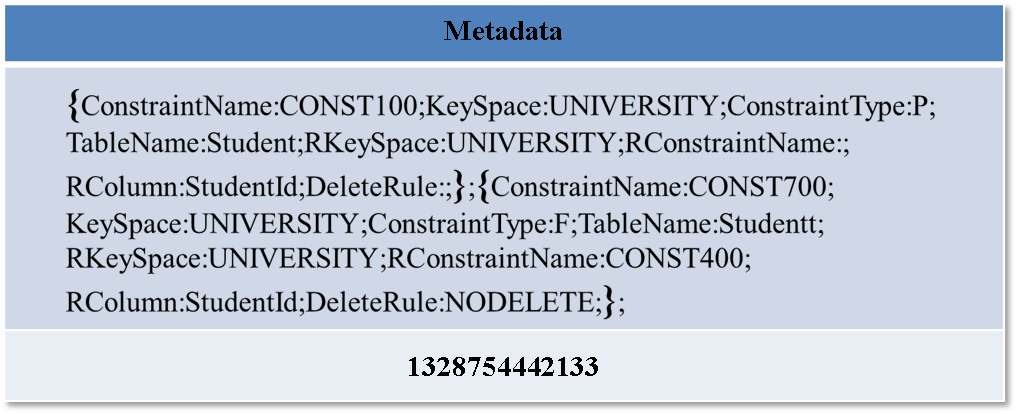
\includegraphics[width=.6\textwidth]{./figure/Solutions/Sol1-MD-Col.png}
	% 			\caption{Response Time for \texttt{insert}}\label{fr:response-insert}
			}
			\subfigure[Metadata in Supercolumns]{
				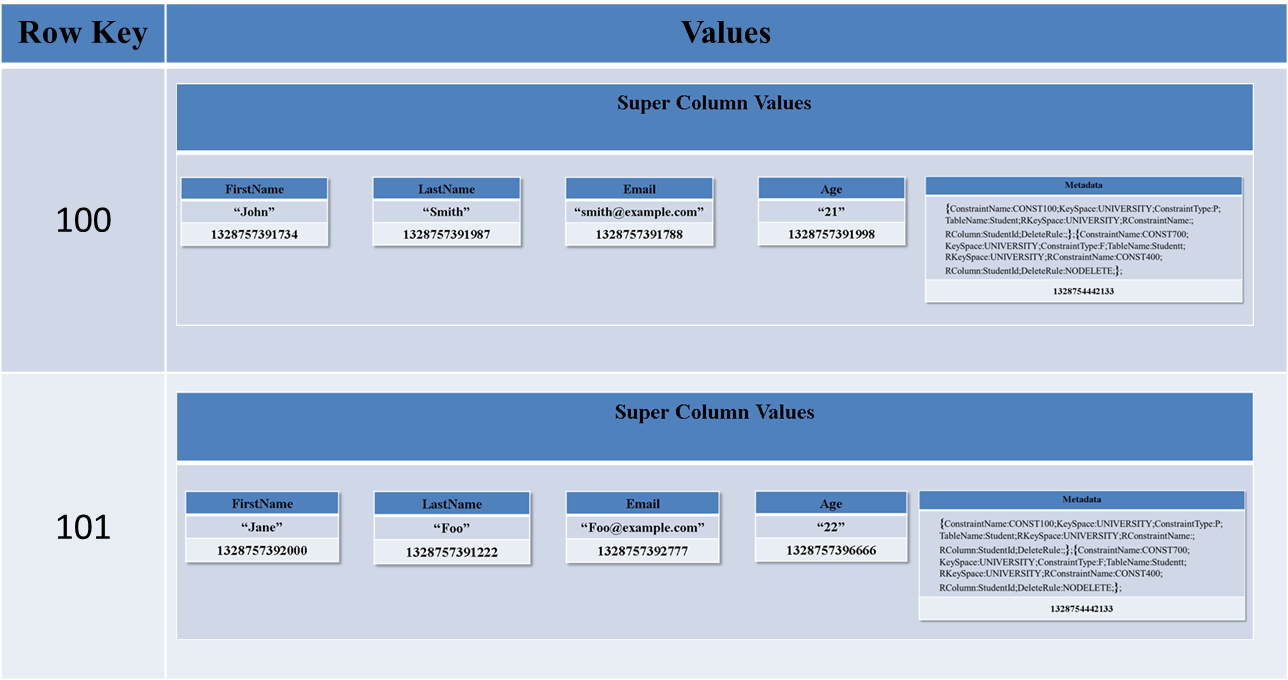
\includegraphics[width=1\textwidth]{./figure/Solutions/Sol1-MD-ColumnFamily.png}
	% 			\caption{Throughput}\label{fr:through-insert}
			} 
			\caption{Metadata storage in Solution 1}
		\end{figure}
Special characters are used within the metadata to separate the constraints and
to identify its different parts. The special characters used in this solution
are '\texttt{\{}', '\texttt{\}}','\texttt{;}' and '\texttt{:}'. The special
characters are used the following way:
	
		\begin{itemize}
			\item Each constraint is enclosed in curly brackets and separated from each
			other by the special character '\texttt{;}'. For example,in \texttt{Student}
			\texttt{CONST100} and \texttt{CONST700} are enclosed in curly braces and
			separated by '\texttt{;}'. Thus, '\texttt{\};}' marks the end of every
			constraint in the metadata.
		
		
			\item The different parts of each constraint are separated by the special character
			'\texttt{;}'. For example,  '\texttt{;}' separates the \texttt{ConstraintName}
			 and \texttt{Keyspace} and other parts in the constraints \texttt{CONST100} and
			 \texttt{CONST700}
			 
			 
			\item Each part and its value are separated by the special character
			'\texttt{:}'. For example, \texttt{ConstraintName} is separated from
			its value \texttt{CONST100} with a \texttt{:}. This helps in identifying the
			name and value for every part while parsing the metadata information
			in the \ac{API}.
			
		\end{itemize}
This metadata is extracted from each super column and processed by specific
methods within the solution so that metadata is used for validating referential
integrity. Different methods are built in the \ac{API} to support these
functionalities and described in the Implementation chapter.

In this solution, the metadata is  repeated several times within the
same column family and due to the replicated nature of the \ac{NoSQL} \acp{DBMS}
the metadata is  stored several times across the nodes in the cluster. This
increases the redundancy of the metadata and much space would be consumed
unnecessarily if the metedata is large. 

This design was inspired by the experiments done on Tokyo Cabinet, a popular
\ac{NoSQL} \ac{DBMS} by Hackl et al.  (2010), where metadata information was
stored as a part of the value in a key-value pair stored in Tokyo Cabinet. In
Hackl et al.  (2010),  metadata management is addressed in the context of huge
file systems, where metadata is stored separately in a suitable \ac{DBMS} so
that such file systems can be managed and administered efficiently without
slowing them down.  To analyse which type of \ac{DBMS} was more suitable for
such a metadata storage,  they conducted various experiments and concluded that
key-value \acp{DBMS} were more efficient in terms of speed,  memory and resource
consumption when compared to popular \acp{RDBMS}.  As a part of their
experiments, they adopted an interesting approach to store metadata in  Tokyo
Cabinet where records are stored as simple key-value
pairs in data files. Unlike Cassandra, Tokyo Cabinet does not involve data types
or columns and column families (\todo{cite}).
In their approach,  metadata about the file system used in their experiment is
inserted as a value which is associated with a unique key and the different
parts of the metadata are separated by semicolons (Hackl et al.  2010).


\section{Solution2:  Metadata as a Top Row} \label{s:design-sol2}


This solution saves the metadata embedded with the actual data and exists in the
same column family as the data. This approach is similar to Solution~1 where
metadata is stored within the same column family. But unlike Solution~1, this
solution saves the metadata only once in the column family as a top row or the
first super column in a column family with the unique \texttt{RowId}
'\texttt{-1}'. This top row has only a single column \texttt{Metadata} 
containign the metadta information and this is  unlike other super columns which
have different columns. The \texttt{Metadata} column is similar to the
Solution~1 as shown in Figure~\ref{fd:Metadata-Solution1} (a). This is possible
since Cassandra allows rows to have different number of columns, as described in Section~\ref{s::key-value-data-model}. Thus, for each entity class, the metadata
exists only once as a single row and is common for all the instances of the
entity.
In the University example  a \texttt{Student} entity has the metadata  stored as
a top row in Figure~\ref{fd:Metadata-Solution2}.
		 
	\begin{figure}[h]  
		\centering 
		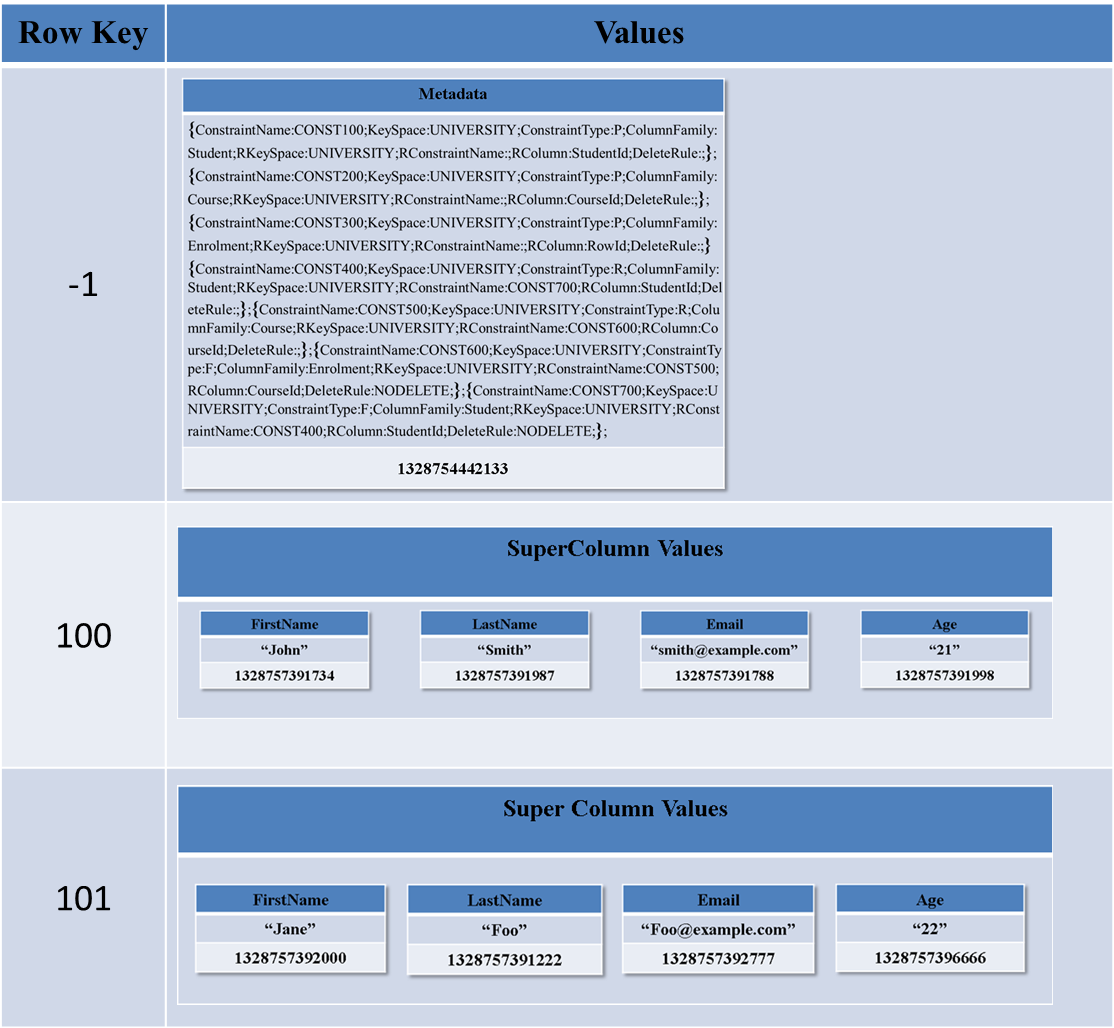
\includegraphics[width=.8\textwidth]{./figure/Solutions/Sol2-MD-ColumnFamily.png}
		\caption{Metadata storage in Solution 2}\label{fd:Metadata-Solution2}
	\end{figure}
		
The metadata in this solution contains special characters '\texttt{\{}',
'\texttt{\}}','\texttt{;}' and '\texttt{:}' to distinguish all the constraints
and its different parts and values.
The metadata stored for each column family has the following constraints:
	\begin{itemize}
	  \item  \ac{PK} constraint showing the primary key of the column family.
	  \item \ac{FK} constraints 
			\begin{itemize}
				\item In the case of a parent entity the \ac{FK} constraints are the \ac{FK}
				constraints of type '\texttt{F}' to identify the child entities when the entity
				is being updated or deleted.
				\item  In the case of a child entity the \ac{FK} constraint of type '\texttt{R}'
				would be stored along with the \ac{PK} constraint which indicates its parent
				entities.
				\item If an entity is both a parent and child entity, then its metadata would
				hold its \ac{PK} constraint, and the \ac{FK} constraints of both types.
			\end{itemize}
	\end{itemize}
	
Consider \texttt{Enrolment}  which is a child entity with parent entities
\texttt{Student} and \texttt{Course} (Figure~\ref{}). Its metadata thus contains
its \ac{PK} constraint \texttt{CONST300} and the \ac{FK} constraints
\texttt{CONST400} and \texttt{CONST500}. Since \texttt{Student} is a child
entity it  stores its \ac{PK} constraint \texttt{CONST100} and its \ac{FK}
constraint \texttt{CONST700}. Similarly, \texttt{Course} stores its \ac{PK} and
respective \ac{FK} constraints.

	\begin{figure}
	\todo{ Insert metadata top row figure for Enrolment}
	\end{figure}
% 	Thus, the metadats describes which is the
% 	primary key for the entity and the \ac{FK} constraints show which child entities dependent on the
% 	entity. The \ac{FK} constraints are particularly useful to .
	
The motivation for this solution was to overcome the redundancy of metadata
storage in Solution~1. In solution~1 metedata was stored in every super column
of a column family and replicated across the cluster along with the column
family. Solution~2 reduces this redundancy and centralises the metedata as a top
row within the column family and is common for all instances in an entity class.
This solution also ensures that when changes have to be made ot the metadata the
actual data is not accessed and only the column family of the data is accessed. 
Moreover when metadata is large, it consumes less space as it is not replicated
as widely as in Solution~1.
In other words, the aim of this design was to reduce the redundancy of metadata
in the column family whilst having metadata accessible to all the nodes by
having it embedded with the actual data.


\section{Solution3:  Metadata Column Family} \label{s:design-sol3}

This solution saves the metadata for all the entities in a separate column
family called \texttt{Metadata}.  In this approach the metadata is
decoupled from the actual data and stored in decentalised way where all the
\ac{PK} and \ac{FK} constraints for all the column famliies within the keyspace
are saved in one location. All the constraints as seen in
Figure~\ref{fd:Metadata-Constraints} are saved as super columns in the
\texttt{Metadata} column family (Figure~\ref{fd:Metadata-Solution3}). 
 
	\begin{figure}[h] 
		\centering
		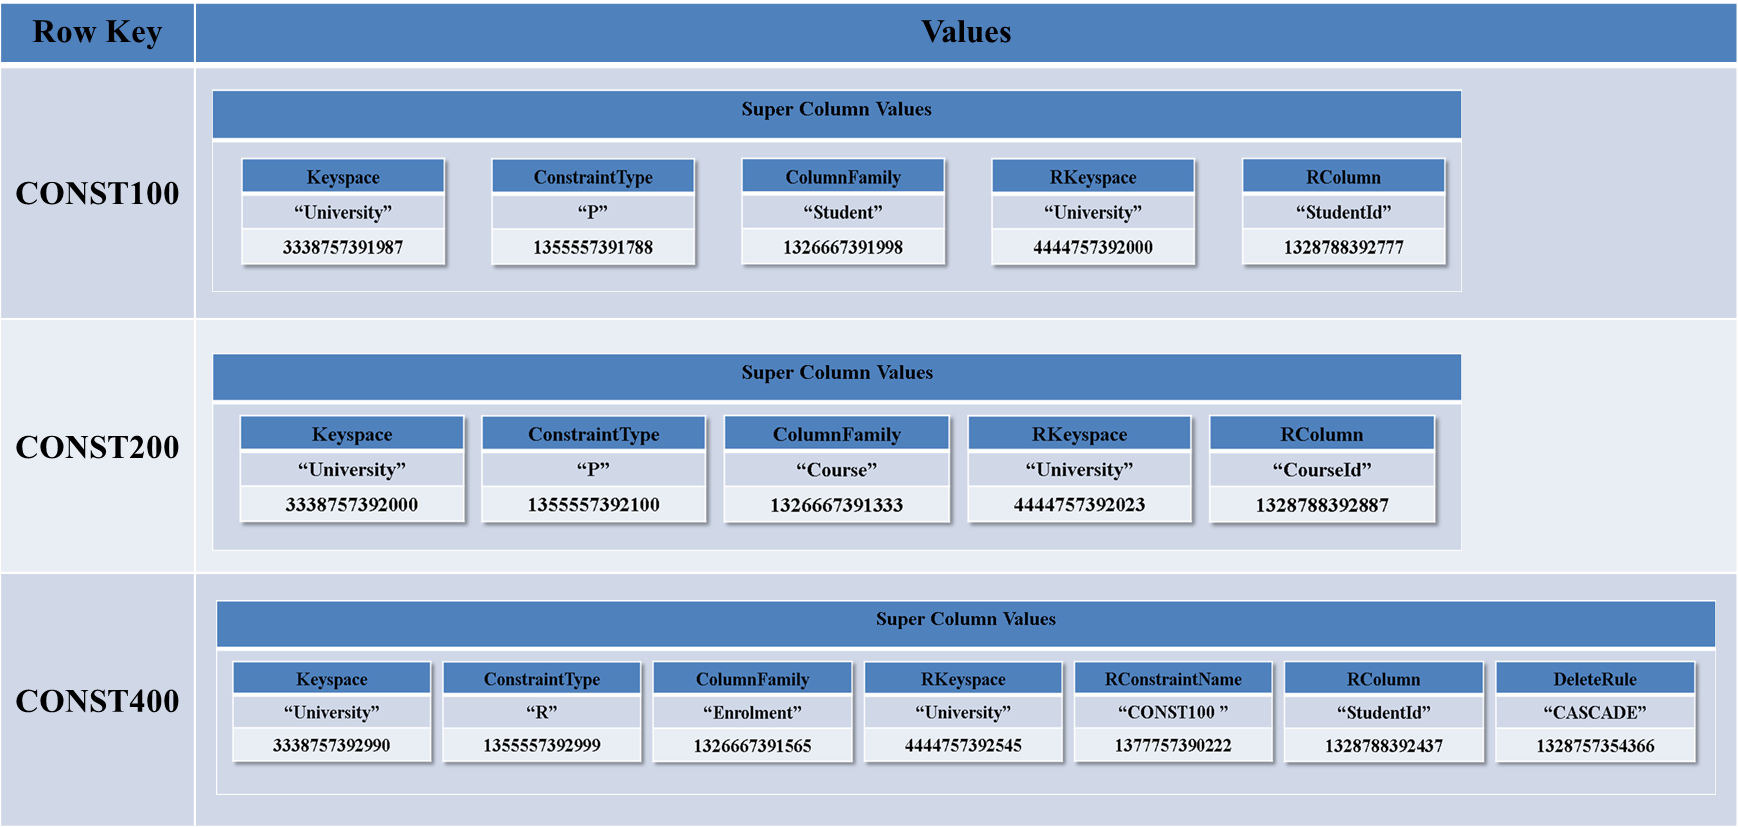
\includegraphics[width=.8\textwidth]{./figure/Solutions/Sol3-MD-ColumnFamily.png}
		\caption{Metadata Column Family in Solution 3}\label{fd:Metadata-Solution3}
	\end{figure}

The different parts of these constraints are saved as separate columns in this
approach and thus no special characters are requireed to identify the various
parts as in Solutions~1 and 2. Thus, for validating referential integruty, the
\ac{API} connects to this column family and retrieves the relevant constraints
for an entity. The different parts are accessed and its values retrived to do
the validation.

This approach is similar to the way dependency information is
stored in traditional \acp{RDBMS}, where metadata holds all the information
about entities and their dependencies and other properties. Commonly such
metadata is maintained separately from the entities in \texttt{System}tables
that can be commonly accessed by the users of the database. 

The design to decouple metadata and the actual data is inspired from the
potential problems and cases where Solutions~1 and 2 could prove to be less
useful. Such cases are when metadata undergoes frequent changes or a column
family has many constraints. When a column family has too many constraints the
value in \texttt{Metadata} column will be too large and accessing as well as
processing the large metadtaa can consume more time. In these designs, to make
changes to metadata it is required that the metadata be changed at every place
it was repeated. This meant that in Solution~1 the \texttt{Metadata} column in
every super column has to be updated every time a constraint is added, removed
or updated. In Solution~2, the top row has to be changed for all the column
famlies that have any alterations  in their constraints.
By decoupling metadtaa from the actual data it is  easier to access and retrieve
the various parts of the constraints since can be searched based on the column
names once the constraint is identified.
More importanlty it is now possible to add or remove constraints for a column
family as it is centrally stored. Any changes to metedata affects only the
\texttt{Metadata} column family and the \ac{API} does not have to access actual
data to perform these changes. 

\section{Solution4:  Metadata Cluster} \label{s:design-sol4}

Similar to Solution 3, metadata in this solution is saved in a separate column
family as shown in Figure~\ref{fd:Metadata-Solution3}. Instead of saving the
metadata as a column family within the same keyspace, it is saved in a separate
Cassandra cluster.This means that the metadata storage is decentralised and separated from the
Cassandra cluster. Metadata  is not as widely replicated as in the previous
solutions since the rpelication of metadata is only within the metadata cluster. 


% The Cassandra cluster is named ‘Test Cluster’ and consists
% of the nodes that have Cassandra with the entity column families (Student,
% Course, and Enrolment). A separate cluster called “Metadata Cluster” consists of
% nodes that have only the metadata column families.
\begin{figure}[h]
	\centering
	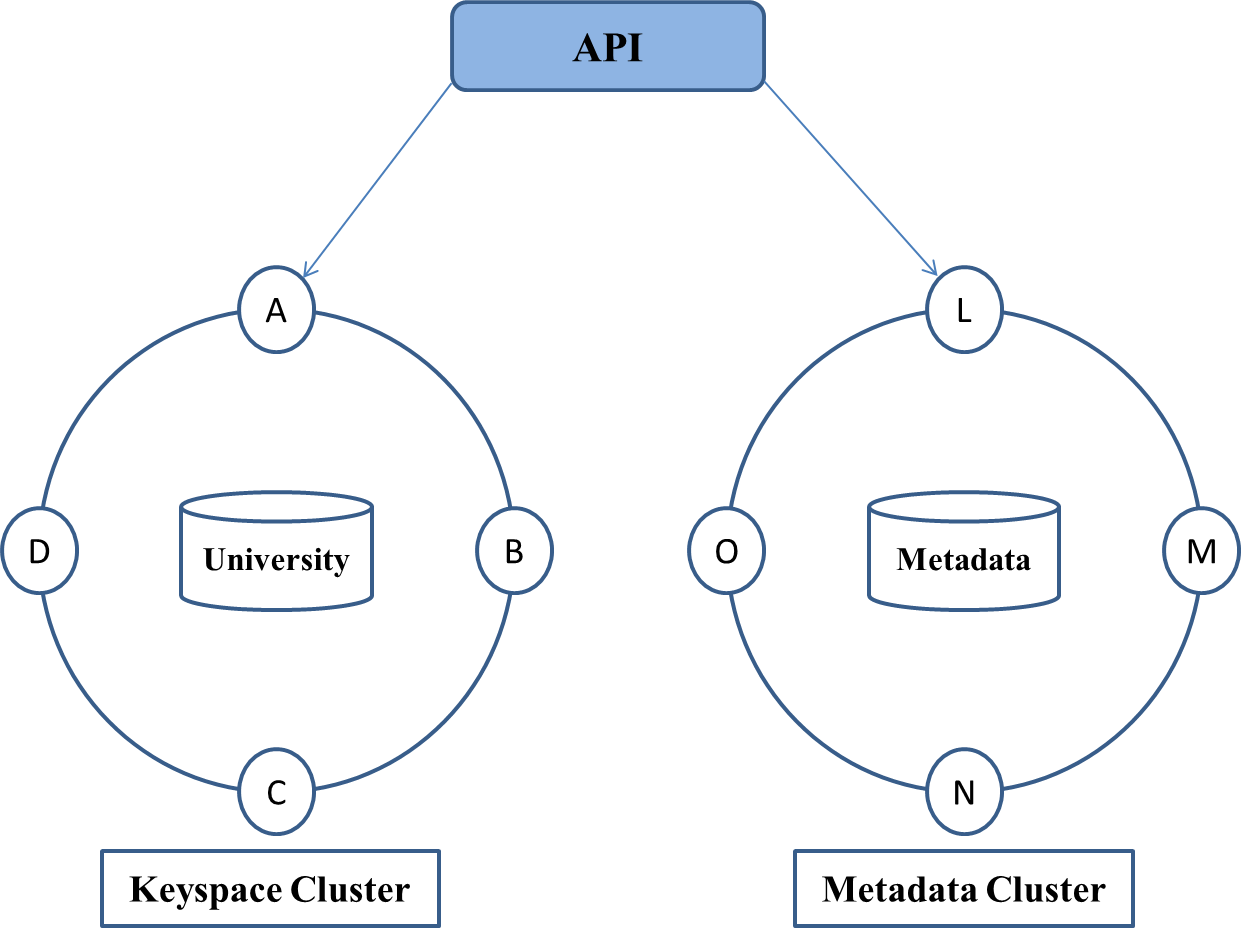
\includegraphics[width=.6\textwidth]{./figure/Solutions/Sol4-cluster-pic.png}
	\caption{Metadata Cluster in Solution
	4}\label{fd:MetadataCluster-Solution4}
	
\end{figure}

The \ac{API} connects to the Metadata cluster as well as the  cluster containing the
keyspace to perform any database operations. Whenever the metadata is
accessed the \ac{API} caches it for processing the
operations on the column famliies and to re-use the metadata. This si also
so that even if the metadata cluster is unresponsive or not active the \ac{API}
can perform operations with the cached metadata. Having metadata in a
persistence layer is effective since metedata is not frequently changed like the
actual data and also saves operational time by not having to connect to the
metadata column family each time  metadata is accessed.


% As of now, ‘Test Cluster’ is the name of the cluster for all the entity column
% families existing on Cassandra nodes. Some of the Cassandra nodes are
% Saddleback, meow, Marrakech etc. located in the ECS labs. To have a separate
% cluster of nodes for Metadata, it was required that the Cassandra configuration
% files were changed. This involved changing the listening port, RPC port, and TCP
% port to different values from that of the ‘Test Cluster’. It was also necessary
% to change the path configurations for the saved caches and log files so that it
% does not overwrite the files of the ‘Test Cluster’.
For example, in Solution 4 the metadata column family \texttt{Metadata} is
inserted into a separate cluster \texttt{MetadataCluster}, while the column
families \texttt{Student}, \texttt{course} and \texttt{Enrolment} are entered
into another cluster.

%  Just as in other solutions, metadata information needs to be checked during any
%  database operations. Every time a referential integrity check is performed, the
%  API connects to the ‘Metadata Cluster’ and retrieves the metadata information.
%  Connection pools are maintained to reuse the connections whenever needed. In
%  order to perform the database operations, the API then connects to the ‘Test
%  Cluster’ on any of its nodes. For example, if an insert operation is invoked on
%  Enrolment, it is necessary to check if the foreign keys for Student and Course
%  column families exist in their respective parent column families. The details
%  of the referenced column families are retrieved from the Metadata column family
%  in the ‘Metadata Cluster’. Once this information is processed, the API connects
%  to the referencing column families in the ‘Test Cluster’ and completes the
%  insert operation.
 Such a design approach is suitable when an application handles multiple
 keyspaces and have to store and maintain metadata for its several keyspaces. In
 these situations it is straightforward and simpler to maintain all the metadata
 in a separate cluster and decoupled form the actual data.  Even if the metadata
 cluster is unresponsive or not active the \ac{API} can perform operations with
 the cached metadata.
 
 This approach is inspired from the way most distributed systems
 save metadata in \ac{MDS} clusters (Lin Xia et al. 2009).
 For better scalability and efficient access of metadata, \ac{MDS} are
 often separate clusters in large distributed environments. In distributed
 systems such clusters  have a master \ac{MDS} and subordinate \acp{MDS}, with
 each server running on a different node. But in this solution such a management
 is not required since in a Cassandra cluster all nodes have the same
 responsibilites and do not have a master-slave configuration.
 
\section{Summary}
The significant difference in the design of all the  solutions is the way each
of the solutions store metedata. While Solution~1 stores metadata with the data
in every super column increasing the redundancy it provides easier access and to the metadata.
Solution~2 addresses reduces the redundancy of metedata and is useful when the
metadata is large for a column family since it consumes lesser space when
compared to Solution~1. Solution~3 separates the metedata from the actual data
and stores all the constraints of all the column famlies in a keyspace together
in a centralised way. This is useful when metadata has to be amended or altered.
Moreover this also removes handling the data each time metadata has to be
accessed. So the operations involving metadata need not have to process the
data. Solution~4 has a similar approach as Solution~3 but saves the metedata
column family in a separate cluster on different nodes. It also introduces
caching the metadata and thus saving oprational time and connections.

The way metadata is retrieved and
processed are different in each of the solutions since the way metadata is
stored is unique in each  solution. Referential integrity validations are
triggered when a \ac{CRUD} operation is performed on a column family. The logic
for validating the referential integrity is consistenst across all the soltuions
and specific methods exist in the \ac{API} to perform these processes. The way
the \ac{API} handles all the \ac{CRUD} operations and the validations that are
triggered during these operations and themetadata retrieval and processing
done in ecah solutions are discussed in detail in
Chapter~\ref{c:Implementation}.
% It also explains how each of the solutions retrieves and processes the metadata.

% The insert, update and delete operations are performed similar to the other
% solutions.


% These methods and all the
% solutions are incorporated  into an experimental \ac{API}, which is
% described in Chapter~\ref{c:Implementation}.
